
%% bare_conf.tex
%% V1.3
%% 2007/01/11
%% by Michael Shell
%% See:
%% http://www.michaelshell.org/
%% for current contact information.
%%
%% This is a skeleton file demonstrating the use of IEEEtran.cls
%% (requires IEEEtran.cls version 1.7 or later) with an IEEE conference paper.
%%
%% Support sites:
%% http://www.michaelshell.org/tex/ieeetran/
%% http://www.ctan.org/tex-archive/macros/latex/contrib/IEEEtran/
%% and
%% http://www.ieee.org/

%%*************************************************************************
%% Legal Notice:
%% This code is offered as-is without any warranty either expressed or
%% implied; without even the implied warranty of MERCHANTABILITY or
%% FITNESS FOR A PARTICULAR PURPOSE! 
%% User assumes all risk.
%% In no event shall IEEE or any contributor to this code be liable for
%% any damages or losses, including, but not limited to, incidental,
%% consequential, or any other damages, resulting from the use or misuse
%% of any information contained here.
%%
%% All comments are the opinions of their respective authors and are not
%% necessarily endorsed by the IEEE.
%%
%% This work is distributed under the LaTeX Project Public License (LPPL)
%% ( http://www.latex-project.org/ ) version 1.3, and may be freely used,
%% distributed and modified. A copy of the LPPL, version 1.3, is included
%% in the base LaTeX documentation of all distributions of LaTeX released
%% 2003/12/01 or later.
%% Retain all contribution notices and credits.
%% ** Modified files should be clearly indicated as such, including  **
%% ** renaming them and changing author support contact information. **
%%
%% File list of work: IEEEtran.cls, IEEEtran_HOWTO.pdf, bare_adv.tex,
%%                    bare_conf.tex, bare_jrnl.tex, bare_jrnl_compsoc.tex
%%*************************************************************************

% *** Authors should verify (and, if needed, correct) their LaTeX system  ***
% *** with the testflow diagnostic prior to trusting their LaTeX platform ***
% *** with production work. IEEE's font choices can trigger bugs that do  ***
% *** not appear when using other class files.                            ***
% The testflow support page is at:
% http://www.michaelshell.org/tex/testflow/



% Note that the a4paper option is mainly intended so that authors in
% countries using A4 can easily print to A4 and see how their papers will
% look in print - the typesetting of the document will not typically be
% affected with changes in paper size (but the bottom and side margins will).
% Use the testflow package mentioned above to verify correct handling of
% both paper sizes by the user's LaTeX system.
%
% Also note that the "draftcls" or "draftclsnofoot", not "draft", option
% should be used if it is desired that the figures are to be displayed in
% draft mode.
%
\documentclass[conference]{IEEEtran}
% Add the compsoc option for Computer Society conferences.
%
% If IEEEtran.cls has not been installed into the LaTeX system files,
% manually specify the path to it like:
% \documentclass[conference]{../sty/IEEEtran}





% Some very useful LaTeX packages include:
% (uncomment the ones you want to load)


% *** MISC UTILITY PACKAGES ***
%
%\usepackage{ifpdf}
% Heiko Oberdiek's ifpdf.sty is very useful if you need conditional
% compilation based on whether the output is pdf or dvi.
% usage:
% \ifpdf
%   % pdf code
% \else
%   % dvi code
% \fi
% The latest version of ifpdf.sty can be obtained from:
% http://www.ctan.org/tex-archive/macros/latex/contrib/oberdiek/
% Also, note that IEEEtran.cls V1.7 and later provides a builtin
% \ifCLASSINFOpdf conditional that works the same way.
% When switching from latex to pdflatex and vice-versa, the compiler may
% have to be run twice to clear warning/error messages.






% *** CITATION PACKAGES ***
%
\usepackage{cite}
% cite.sty was written by Donald Arseneau
% V1.6 and later of IEEEtran pre-defines the format of the cite.sty package
% \cite{} output to follow that of IEEE. Loading the cite package will
% result in citation numbers being automatically sorted and properly
% "compressed/ranged". e.g., [1], [9], [2], [7], [5], [6] without using
% cite.sty will become [1], [2], [5]--[7], [9] using cite.sty. cite.sty's
% \cite will automatically add leading space, if needed. Use cite.sty's
% noadjust option (cite.sty V3.8 and later) if you want to turn this off.
% cite.sty is already installed on most LaTeX systems. Be sure and use
% version 4.0 (2003-05-27) and later if using hyperref.sty. cite.sty does
% not currently provide for hyperlinked citations.
% The latest version can be obtained at:
% http://www.ctan.org/tex-archive/macros/latex/contrib/cite/
% The documentation is contained in the cite.sty file itself.






% *** GRAPHICS RELATED PACKAGES ***
%
\ifCLASSINFOpdf
  % \usepackage[pdftex]{graphicx}
  % declare the path(s) where your graphic files are
  % \graphicspath{{../pdf/}{../jpeg/}}
  % and their extensions so you won't have to specify these with
  % every instance of \includegraphics
  % \DeclareGraphicsExtensions{.pdf,.jpeg,.png}
\else
  % or other class option (dvipsone, dvipdf, if not using dvips). graphicx
  % will default to the driver specified in the system graphics.cfg if no
  % driver is specified.
  % \usepackage[dvips]{graphicx}
  % declare the path(s) where your graphic files are
  % \graphicspath{{../eps/}}
  % and their extensions so you won't have to specify these with
  % every instance of \includegraphics
  % \DeclareGraphicsExtensions{.eps}
\fi
% graphicx was written by David Carlisle and Sebastian Rahtz. It is
% required if you want graphics, photos, etc. graphicx.sty is already
% installed on most LaTeX systems. The latest version and documentation can
% be obtained at: 
% http://www.ctan.org/tex-archive/macros/latex/required/graphics/
% Another good source of documentation is "Using Imported Graphics in
% LaTeX2e" by Keith Reckdahl which can be found as epslatex.ps or
% epslatex.pdf at: http://www.ctan.org/tex-archive/info/
%
% latex, and pdflatex in dvi mode, support graphics in encapsulated
% postscript (.eps) format. pdflatex in pdf mode supports graphics
% in .pdf, .jpeg, .png and .mps (metapost) formats. Users should ensure
% that all non-photo figures use a vector format (.eps, .pdf, .mps) and
% not a bitmapped formats (.jpeg, .png). IEEE frowns on bitmapped formats
% which can result in "jaggedy"/blurry rendering of lines and letters as
% well as large increases in file sizes.
%
% You can find documentation about the pdfTeX application at:
% http://www.tug.org/applications/pdftex





% *** MATH PACKAGES ***
%
%\usepackage[cmex10]{amsmath}
% A popular package from the American Mathematical Society that provides
% many useful and powerful commands for dealing with mathematics. If using
% it, be sure to load this package with the cmex10 option to ensure that
% only type 1 fonts will utilized at all point sizes. Without this option,
% it is possible that some math symbols, particularly those within
% footnotes, will be rendered in bitmap form which will result in a
% document that can not be IEEE Xplore compliant!
%
% Also, note that the amsmath package sets \interdisplaylinepenalty to 10000
% thus preventing page breaks from occurring within multiline equations. Use:
%\interdisplaylinepenalty=2500
% after loading amsmath to restore such page breaks as IEEEtran.cls normally
% does. amsmath.sty is already installed on most LaTeX systems. The latest
% version and documentation can be obtained at:
% http://www.ctan.org/tex-archive/macros/latex/required/amslatex/math/





% *** SPECIALIZED LIST PACKAGES ***
%
%\usepackage{algorithmic}
% algorithmic.sty was written by Peter Williams and Rogerio Brito.
% This package provides an algorithmic environment fo describing algorithms.
% You can use the algorithmic environment in-text or within a figure
% environment to provide for a floating algorithm. Do NOT use the algorithm
% floating environment provided by algorithm.sty (by the same authors) or
% algorithm2e.sty (by Christophe Fiorio) as IEEE does not use dedicated
% algorithm float types and packages that provide these will not provide
% correct IEEE style captions. The latest version and documentation of
% algorithmic.sty can be obtained at:
% http://www.ctan.org/tex-archive/macros/latex/contrib/algorithms/
% There is also a support site at:
% http://algorithms.berlios.de/index.html
% Also of interest may be the (relatively newer and more customizable)
% algorithmicx.sty package by Szasz Janos:
% http://www.ctan.org/tex-archive/macros/latex/contrib/algorithmicx/

%\usepackage[spanish]{babel}
\usepackage[latin1]{inputenc}
%\usepackage[T1]{fontenc}
\usepackage{graphicx}
%\usepackage{float}
\usepackage{alltt}

\usepackage{fancyhdr}
\pagestyle{fancy}

\renewcommand{\figurename}{Figure}
\renewcommand{\tablename}{Table}
\renewcommand{\footnoterule}{\vspace*{-3pt}
  \noindent\rule{5cm}{1pt}\vspace*{2.6pt}}
%\renewcommand{\thesubsection}{\Roman{subsection}: }

% *** ALIGNMENT PACKAGES ***
%
\usepackage{array}
\usepackage{multirow}

% Frank Mittelbach's and David Carlisle's array.sty patches and improves
% the standard LaTeX2e array and tabular environments to provide better
% appearance and additional user controls. As the default LaTeX2e table
% generation code is lacking to the point of almost being broken with
% respect to the quality of the end results, all users are strongly
% advised to use an enhanced (at the very least that provided by array.sty)
% set of table tools. array.sty is already installed on most systems. The
% latest version and documentation can be obtained at:
% http://www.ctan.org/tex-archive/macros/latex/required/tools/


\usepackage{mdwmath}
%\usepackage{mdwtab}
% Also highly recommended is Mark Wooding's extremely powerful MDW tools,
% especially mdwmath.sty and mdwtab.sty which are used to format equations
% and tables, respectively. The MDWtools set is already installed on most
% LaTeX systems. The lastest version and documentation is available at:
% http://www.ctan.org/tex-archive/macros/latex/contrib/mdwtools/


% IEEEtran contains the IEEEeqnarray family of commands that can be used to
% generate multiline equations as well as matrices, tables, etc., of high
% quality.


%\usepackage{eqparbox}
% Also of notable interest is Scott Pakin's eqparbox package for creating
% (automatically sized) equal width boxes - aka "natural width parboxes".
% Available at:
% http://www.ctan.org/tex-archive/macros/latex/contrib/eqparbox/





% *** SUBFIGURE PACKAGES ***
%\usepackage[tight,footnotesize]{subfigure}
% subfigure.sty was written by Steven Douglas Cochran. This package makes it
% easy to put subfigures in your figures. e.g., "Figure 1a and 1b". For IEEE
% work, it is a good idea to load it with the tight package option to reduce
% the amount of white space around the subfigures. subfigure.sty is already
% installed on most LaTeX systems. The latest version and documentation can
% be obtained at:
% http://www.ctan.org/tex-archive/obsolete/macros/latex/contrib/subfigure/
% subfigure.sty has been superceeded by subfig.sty.



%\usepackage[caption=false]{caption}
%\usepackage[font=footnotesize]{subfig}
% subfig.sty, also written by Steven Douglas Cochran, is the modern
% replacement for subfigure.sty. However, subfig.sty requires and
% automatically loads Axel Sommerfeldt's caption.sty which will override
% IEEEtran.cls handling of captions and this will result in nonIEEE style
% figure/table captions. To prevent this problem, be sure and preload
% caption.sty with its "caption=false" package option. This is will preserve
% IEEEtran.cls handing of captions. Version 1.3 (2005/06/28) and later 
% (recommended due to many improvements over 1.2) of subfig.sty supports
% the caption=false option directly:
%\usepackage[caption=false,font=footnotesize]{subfig}
%
% The latest version and documentation can be obtained at:
% http://www.ctan.org/tex-archive/macros/latex/contrib/subfig/
% The latest version and documentation of caption.sty can be obtained at:
% http://www.ctan.org/tex-archive/macros/latex/contrib/caption/




% *** FLOAT PACKAGES ***
%
%\usepackage{fixltx2e}
% fixltx2e, the successor to the earlier fix2col.sty, was written by
% Frank Mittelbach and David Carlisle. This package corrects a few problems
% in the LaTeX2e kernel, the most notable of which is that in current
% LaTeX2e releases, the ordering of single and double column floats is not
% guaranteed to be preserved. Thus, an unpatched LaTeX2e can allow a
% single column figure to be placed prior to an earlier double column
% figure. The latest version and documentation can be found at:
% http://www.ctan.org/tex-archive/macros/latex/base/



%\usepackage{stfloats}
% stfloats.sty was written by Sigitas Tolusis. This package gives LaTeX2e
% the ability to do double column floats at the bottom of the page as well
% as the top. (e.g., "\begin{figure*}[!b]" is not normally possible in
% LaTeX2e). It also provides a command:
%\fnbelowfloat
% to enable the placement of footnotes below bottom floats (the standard
% LaTeX2e kernel puts them above bottom floats). This is an invasive package
% which rewrites many portions of the LaTeX2e float routines. It may not work
% with other packages that modify the LaTeX2e float routines. The latest
% version and documentation can be obtained at:
% http://www.ctan.org/tex-archive/macros/latex/contrib/sttools/
% Documentation is contained in the stfloats.sty comments as well as in the
% presfull.pdf file. Do not use the stfloats baselinefloat ability as IEEE
% does not allow \baselineskip to stretch. Authors submitting work to the
% IEEE should note that IEEE rarely uses double column equations and
% that authors should try to avoid such use. Do not be tempted to use the
% cuted.sty or midfloat.sty packages (also by Sigitas Tolusis) as IEEE does
% not format its papers in such ways.





% *** PDF, URL AND HYPERLINK PACKAGES ***
%
\usepackage{url}
% url.sty was written by Donald Arseneau. It provides better support for
% handling and breaking URLs. url.sty is already installed on most LaTeX
% systems. The latest version can be obtained at:
% http://www.ctan.org/tex-archive/macros/latex/contrib/misc/
% Read the url.sty source comments for usage information. Basically,
% \url{my_url_here}.





% *** Do not adjust lengths that control margins, column widths, etc. ***
% *** Do not use packages that alter fonts (such as pslatex).         ***
% There should be no need to do such things with IEEEtran.cls V1.6 and later.
% (Unless specifically asked to do so by the journal or conference you plan
% to submit to, of course. )


% correct bad hyphenation here
\hyphenation{op-tical net-works semi-conduc-tor}


\begin{document}
%
% paper title
% can use linebreaks \\ within to get better formatting as desired
\title{Integration of Resources for Corporate Memory using Semantic Technologies}


% author names and affiliations
% use a multiple column layout for up to three different
% affiliations
\author{\IEEEauthorblockN{Erik Alarc�n-Zamora}
\IEEEauthorblockA{Department of Electric Engineering\\
Autonomous Metropolitan University\\
Iztapalapa, Mexico\\
Email: cbi2113802469@xanum.uam.mx}
\and
\IEEEauthorblockN{R. Carolina Medina-Ram�rez}
\IEEEauthorblockA{Department of Electric Engineering\\
Autonomous Metropolitan University\\
Iztapalapa, Mexico\\
Email: cmed@xanum.uam.mx}
\and
\IEEEauthorblockN{H�ctor P�rez-Urbina}
\IEEEauthorblockA{Clark \& Parsia, LLC\\
Washington, USA\\
Email: hector@clarkparsia.com}}

% conference papers do not typically use \thanks and this command
% is locked out in conference mode. If really needed, such as for
% the acknowledgment of grants, issue a \IEEEoverridecommandlockouts
% after \documentclass

% for over three affiliations, or if they all won't fit within the width
% of the page, use this alternative format:
% 
%\author{\IEEEauthorblockN{Michael Shell\IEEEauthorrefmark{1},
%Homer Simpson\IEEEauthorrefmark{2},
%James Kirk\IEEEauthorrefmark{3}, 
%Montgomery Scott\IEEEauthorrefmark{3} and
%Eldon Tyrell\IEEEauthorrefmark{4}}
%\IEEEauthorblockA{\IEEEauthorrefmark{1}School of Electrical and Computer Engineering\\
%Georgia Institute of Technology,
%Atlanta, Georgia 30332--0250\\ Email: see http://www.michaelshell.org/contact.html}
%\IEEEauthorblockA{\IEEEauthorrefmark{2}Twentieth Century Fox, Springfield, USA\\
%Email: homer@thesimpsons.com}
%\IEEEauthorblockA{\IEEEauthorrefmark{3}Starfleet Academy, San Francisco, California 96678-2391\\
%Telephone: (800) 555--1212, Fax: (888) 555--1212}
%\IEEEauthorblockA{\IEEEauthorrefmark{4}Tyrell Inc., 123 Replicant Street, Los Angeles, California 90210--4321}}




% use for special paper notices
%\IEEEspecialpapernotice{(Invited Paper)}




% make the title area
\maketitle

\begin{abstract}
%\boldmath
In this paper, we present a framework supported by semantic technologies for integration of the resources of a corporate memory. We describe the methodology adopted for integration of resources as well as a prototype which shows viability of the semantic approach.
\end{abstract}
% IEEEtran.cls defaults to using nonbold math in the Abstract.
% This preserves the distinction between vectors and scalars. However,
% if the conference you are submitting to favors bold math in the abstract,
% then you can use LaTeX's standard command \boldmath at the very start
% of the abstract to achieve this. Many IEEE journals/conferences frown on
% math in the abstract anyway.

% no keywords




% For peer review papers, you can put extra information on the cover
% page as needed:
% \ifCLASSOPTIONpeerreview
% \begin{center} \bfseries EDICS Category: 3-BBND \end{center}
% \fi
%
% For peerreview papers, this IEEEtran command inserts a page break and
% creates the second title. It will be ignored for other modes.
\IEEEpeerreviewmaketitle

\section{Introduction}
\label{sec:intro}
An organization has a wide variety of information resources, such as staff of the organization, databases, electronic documents, reports, books, presentations, videos, etc.. These resources represent knowledge of the organization: products, research, production processes, operational solutions, workflows, objectives, goals, among others. This knowledge is called corporate memory (CM) or organizational memory (OM) and is defined as "\textit{explicit representation, consistent and persistent knowledge in an organization}" \cite{Corpmem98}. A memory is important for persons enrolled (members) or people interested in the organization, because it allows them to access, share, exchange and reuse knowledge. Given the importance of memory, you need knowledge management of the same, in order to have the following advantages: better informed staff, better communication in the organization, better decision making, a support tool for learning , a knowledge base persistent and accessible, a tool to search, retrieval and knowledge sharing, to name a few.

Semantic technologies (TS) \cite{SemTecRetr} are \textit{a set of methodologies, languages, applications, tools and standards to provide or obtain the meaning of the information} \footnote{L. Feigenbaum, ``Semantic Web vs. Semantic Technologies,'' Available: \url{http://www.cambridgesemantics.com/semantic-university/semantic-web-vs-semantic-technologies}}. These technologies add a \textit{abstraction layer} on sources of information, so that the automatic processes to access, process, reason, combine, reuse and share information. The benefits of using semantic technologies are: catch the vision of contexts, adapting to the changing nature of knowledge, considering the distributed nature of knowledge and users, integrate information from different sources, modeling information in a format standard, use a flexible data model, remove ambiguities in the model, inferences about knowledge, develop generic applications, deploy at lower cost and greater interaction of the experts in the domain.

Semantic technologies can represent and manage knowledge in a corporate memory. In particular, let you do the integration process (search and retrieval) significant information resources in a corporate memory. To achieve this integration, you must carry out the following activities: \textit{1) model the knowledge of resources in a standard format, 2) exploit the implicit knowledge of resources and describe vocabulary (concepts and relationships) from memory}, and \textit{3) search and retrieve information on resources, to answer a given question.}

A corporate memory has multiple information resources and for limiting them to a manageable set, we analyze for detecting priority use cases. This article describes two basic use cases that can be employed in any corporate memory:

\begin{enumerate}
	\item\textbf{\textit{Competency Cartography}}: is the search and recovery of significant information of individuals, from the personal and professional characteristics of the same. Some of these professional features are: \textit{skills} (ability to work in a team, leadership skills, etc.), \textit{language skills} (read English, write in Spanish, speaking in French, etc..), \textit{knowledge in the areas of corporate memory domain} (eg operating systems, cognitive radios, etc..), among others.
	\item\textbf{\textit{Search Digital Resources}}: involves the search and retrieval of meaningful information from documents and media files from the content thereof. Some of the search parameters of these resources are: \textit{the author} extension (pdf, doc, wav, etc.), \textit{the issues is the resource} (eg operating systems, ontologies, cognitive radios, etc.), among others.
\end{enumerate}

In this article, represents and integrates corporate memory of \textit{Area Networks \& Telecommunications (R\&T) of the Autonomous Metropolitan University (UAM)}. The resources of this report represent knowledge of teacher-researchers of R\&T. In particular, represent their research resources, collaborations, projects, courses and topics of interest.

This article is organized as follows: section \ref{sec:isr} presents our methodology for semantic integration of resources in a corporate memory. This section is divided into six subsections. Subsection \ref{sec:prop} generally describing the methodology and the three general stages of it (representation, development and consultation of the knowledge of resources). Subsection \ref{sec:arch} shows the architecture for semantic integration. Subsection \ref{sec:rep} describes the resource description framework (RDF) to represent (model) explicit knowledge of resources. Subsection \ref{sec:expl} describes axioms and the way to exploit implicit knowledge of resources. Subsection \ref{sec:cons} explains query language to interrogate knowledge in the model. Subsection \ref{sec:proto} describes the purpose of the prototype for semantic integration. In Section \ref{sec:exp} describes the tests and results (performance and quality of responses) that were made to triplestore Jena \footnote{The Apache Software Foundation, ``Apache Jena'', Available: \url{http://jena.apache.org/}} and the model for the \textit{networks \& telecommunications}. Finally, conclusions about the semantic integration of resources and the experimental results are presented in section \ref{sec:concl}.

% An example of a floating figure using the graphicx package.
% Note that \label must occur AFTER (or within) \caption.
% For figures, \caption should occur after the \includegraphics.
% Note that IEEEtran v1.7 and later has special internal code that
% is designed to preserve the operation of \label within \caption
% even when the captionsoff option is in effect. However, because
% of issues like this, it may be the safest practice to put all your
% \label just after \caption rather than within \caption{}.
%
% Reminder: the "draftcls" or "draftclsnofoot", not "draft", class
% option should be used if it is desired that the figures are to be
% displayed while in draft mode.
%
%\begin{figure}[!t]
%\centering
%\includegraphics[width=2.5in]{myfigure}
% where an .eps filename suffix will be assumed under latex, 
% and a .pdf suffix will be assumed for pdflatex; or what has been declared
% via \DeclareGraphicsExtensions.
%\caption{Simulation Results}
%\label{fig_sim}
%\end{figure}

% Note that IEEE typically puts floats only at the top, even when this
% results in a large percentage of a column being occupied by floats.


% An example of a double column floating figure using two subfigures.
% (The subfig.sty package must be loaded for this to work.)
% The subfigure \label commands are set within each subfloat command, the
% \label for the overall figure must come after \caption.
% \hfil must be used as a separator to get equal spacing.
% The subfigure.sty package works much the same way, except \subfigure is
% used instead of \subfloat.
%
%\begin{figure*}[!t]
%\centerline{\subfloat[Case I]\includegraphics[width=2.5in]{subfigcase1}%
%\label{fig_first_case}}
%\hfil
%\subfloat[Case II]{\includegraphics[width=2.5in]{subfigcase2}%
%\label{fig_second_case}}}
%\caption{Simulation results}
%\label{fig_sim}
%\end{figure*}
%
% Note that often IEEE papers with subfigures do not employ subfigure
% captions (using the optional argument to \subfloat), but instead will
% reference/describe all of them (a), (b), etc., within the main caption.


% An example of a floating table. Note that, for IEEE style tables, the 
% \caption command should come BEFORE the table. Table text will default to
% \footnotesize as IEEE normally uses this smaller font for tables.
% The \label must come after \caption as always.
%
%\begin{table}[!t]
%% increase table row spacing, adjust to taste
%\renewcommand{\arraystretch}{1.3}
% if using array.sty, it might be a good idea to tweak the value of
% \extrarowheight as needed to properly center the text within the cells
%\caption{An Example of a Table}
%\label{table_example}
%\centering
%% Some packages, such as MDW tools, offer better commands for making tables
%% than the plain LaTeX2e tabular which is used here.
%\begin{tabular}{|c||c|}
%\hline
%One & Two\\
%\hline
%Three & Four\\
%\hline
%\end{tabular}
%\end{table}


% Note that IEEE does not put floats in the very first column - or typically
% anywhere on the first page for that matter. Also, in-text middle ("here")
% positioning is not used. Most IEEE journals/conferences use top floats
% exclusively. Note that, LaTeX2e, unlike IEEE journals/conferences, places
% footnotes above bottom floats. This can be corrected via the \fnbelowfloat
% command of the stfloats package.
\section{Semantic Integration Resources}
\label{sec:isr}
Semantic Integration Resource (SIR) is the process of search and retrieval of information significant existing information resources (documents) that are resident on a storage medium. It is based on the use of semantic technologies (ST)\cite{SemTecConc}. The purpose of this integration is to retrieve documents related to answer a question asked by a user. In this paper, integration SIR is effected in a corporate memory (CM), because this SIR considers some important features of a corporate memory as: explosive growth of resources, heterogeneity in format, content and structure of resources, ambiguities in the information, evolution of knowledge about resources (add, delete, or amend), among others. The main users in the ISR are the experts and people linked to the domain of the CM. In the following subsections, we describe our proposed integration and architecture of this, a knowledge representation of resources, how to exploit knowledge of resources, searching for information, as well as an interface prototype.
\subsection{Proposal}
\label{sec:prop}
We propose a methodology for developing \textit{semantic integration of resources} in a \textit{corporate memory}. This methodology was developed considering two use cases, but can be extended to other use cases. This methodology can be used in any CM, for example, Biomedical, Networks and Telecommunications, Chemistry, Biology, Physics, among others, since these are composed of information resources that can be integrated to answer user questions. To carry out the  SIR, our methodology involves three general stages:
\begin{enumerate}
    \item Knowledge Representation: consists in modeling the explicit knowledge of resources in a standard format.
    \item Knowledge Exploitation: consists in using inference rules to materialize implicit knowledge.
    \item Information Query: involves interrogating the knowledge model from a user a question and respond with information about the resources.
\end{enumerate}

\subsection{Architecture}
\label{sec:arq}
The proposed architecture for semantic integration is a solution, which on the one hand, represents and exploits knowledge about the resources of a corporate memory in a model, on the other hand, allows the integration (search and retrieval of information) on the model knowledge. This architecture is generic and can be implemented in any corporate memory associated with a domain. Figure \ref{fig:arq} shows our architecture, in which several components are developed in one of three stages of the SIR.
\begin{figure}[htb]
\centering
%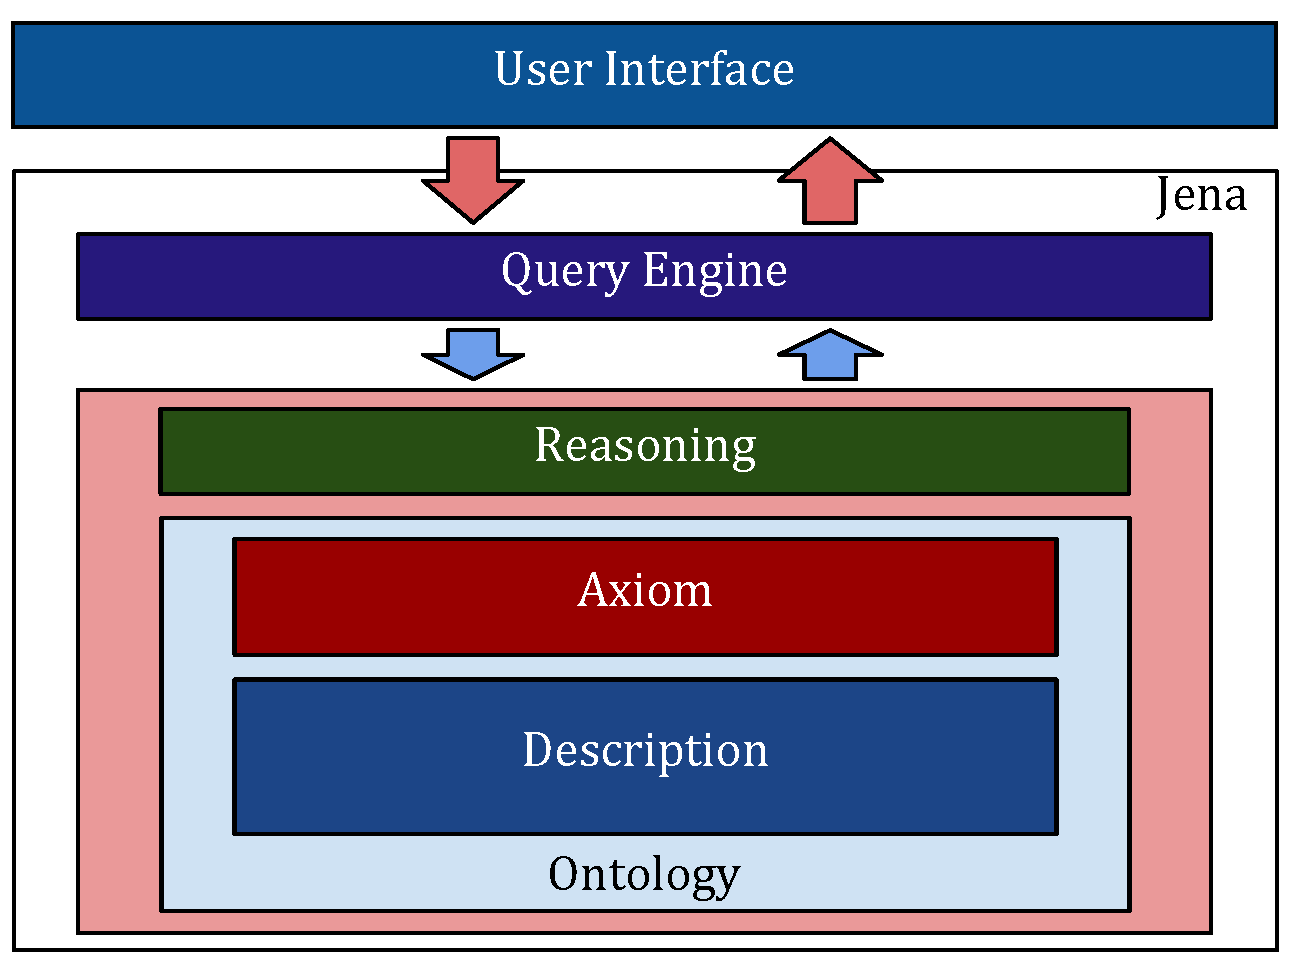
\includegraphics[width=3.2in]{Arquitectura}
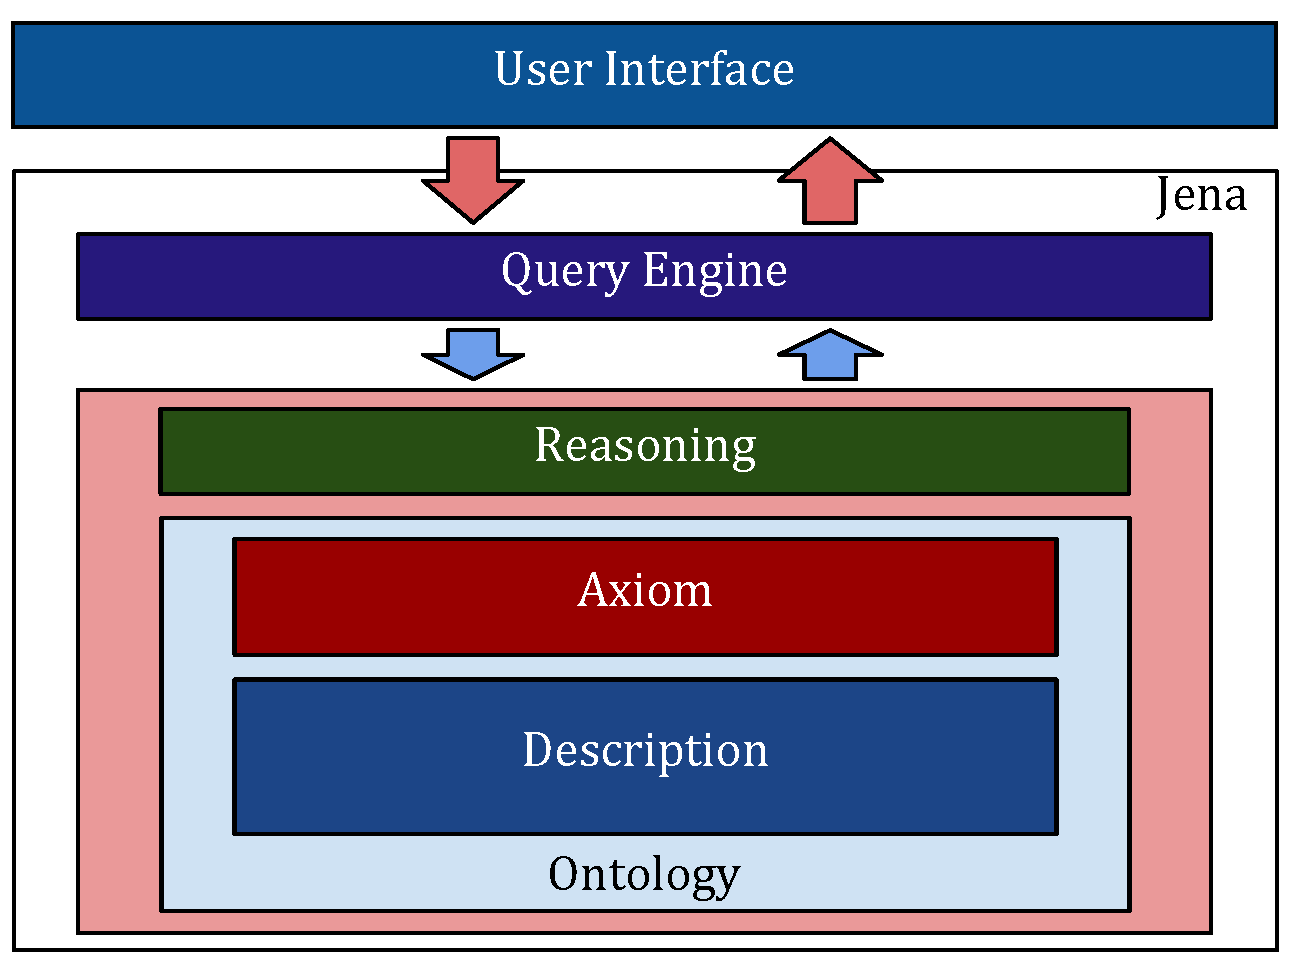
\includegraphics[height=2.2in,width=3.2in]{Arquitectura}
\caption{General architecture for semantic integration of resources on a corporate memory}
\label{fig:arq}
\end{figure}

\subsection{Knowledge Representation}
\label{sec:rep}
In semantic technologies, it has the framework RDF (Resource Descrption Framework\footnote{W3C,``RDF 1.1 Concepts and Abstract Syntax,'' Available: \url{http://www.w3.org/TR/rdf11-concepts/}}) for knowledge representation of resources in a standard format \cite{SurvSemWeb2012}. The first step to represent the RDF Framework, is established to each resource corporate memory one Resource Unique Identifier  \cite{rfc3986} (URI), in order that every resource has a unique name and there is no ambiguity between them. For example, the resource \textit{Towards a semantic search} is assigned the following name: \textit{\url{http://arte.izt.uam.mx/ontologies/digiResourceRyT.owl}\#Hacia\_busqueda\_semantica}.

Within the framework RDF, resources are represented by their properties (basic characteristics or metadata) and the values assigned to them; this representation is also known as resource description. Each property (title, author and source language) has a unique identifier (URI) as a name. In writing of the name, a verb is written in third person and present tense (`Is', `is',`known',  among others) before metadata. For example, the property \textit{title} has the following URI:  \textit{\url{http://arte.izt.uam.mx/ontologies/digiResourceRyT.owl}\#has-title}.

To reduce the size of the identifier (URI) of resources and properties, is replaced sequence of characters from \textit{\url{http://www}} to the symbol \textit{\#} for a certain prefix. In our case study the prefix \textit{sirp} translates \textit{\url{http://arte.izt.uam.mx/ontologies/digiResourceRyT.owl}\#}. For example, the property \textit{has title} is written \textit{sirp: has-title}. In semantic technologies, other prefixes assigned to other vocabularies, such as \textit{rdf, xsd, rdfs and owl}.

The resource properties and their values are taken to a standard format, which in this framework is called triple \cite{SurvSemWeb2012}. The set of all RDF triples on the resources of a domain, is called assertive component (ABox) \cite{Markus2012DLprimer}. A triple is formed by a subject, a predicate and an object; subject is identifier of a resource being described, predicate is identifier of a property described, and the object is either a literal (string, integer) or other resource identifier. An important property for a resource is \textit{assignment}, which links to the resource with a particular class. In the case study, digital resources in the \textbf{\textit{CM of N\&T}} are classified as: Article, Technical Report, Website, Thesis, Book, Slideshow, Image, Audio and Video. In the representation of this \textit{assignment} in the form of RDF triple; subject is a resource, predicate is the name of the assignment (belonging) in the RDF vocabulary is defined as \textit{rdf:type}, and the object is a identifier of a class. For example, the description \textit{Towards a Semantic Search is an article}, is written in triple as follows: sirp:Hacia\_busqueda\_semantica rdf:type sirp:Article.

There are different way of writing triples from the manual, writing literals and identifiers in a text editor, to automated, using tools to map the information to triples \cite{Corcho:2006}, \cite{Uren:2006}, \cite{Han:2008}, as: OntoMat, MnM, GATE, KIM, Media and RDF123 Aktive. In this paper, the tool we choose is the triplestore \textit{Apache Jena} \cite{McBride}, because it provides reading, processing and writing triples in different formats (XML/RDF, N-triples, Turtle), and this triplestore can be used with the programming language \textit{JAVA}. A triplestore is a system that has two basic functions: the storage and access of RDF triples. There are other triplestore \cite{2013interlinking}, \cite{MuhleisenWT11} as: Stardog, 4store, OWLIM, Sesame, among others.

\subsection{Knowledge Explosion}
\label{sec:expl}
At this point, the RDF framework or model to represent explicit knowledge of the resources (data model). This model can be enriched with introduction of \textit{axioms} \cite{DesLog} which supplement, extend, renew and adapt knowledge of resources. To identify the axioms, we analyze the classes/properties and ask questions about them: what classes can be grouped under another class, which properties are grouped under other property, which are disjoint classes, which are synonymous or equivalents classes, what classes or class-literal relates a property, which properties are equivalents (synonymous), property is symmetric, transitive or reflexive, just to mention a few questions.For our case study, we use the following axioms:

\textbf{Subclass and Subproperty},  allow establishing hierarchies among classes (Figure \ref{fig:jcl}) and properties (Figure \ref{fig:jpr}) respectively.

\begin{figure}[!htb]
\centering
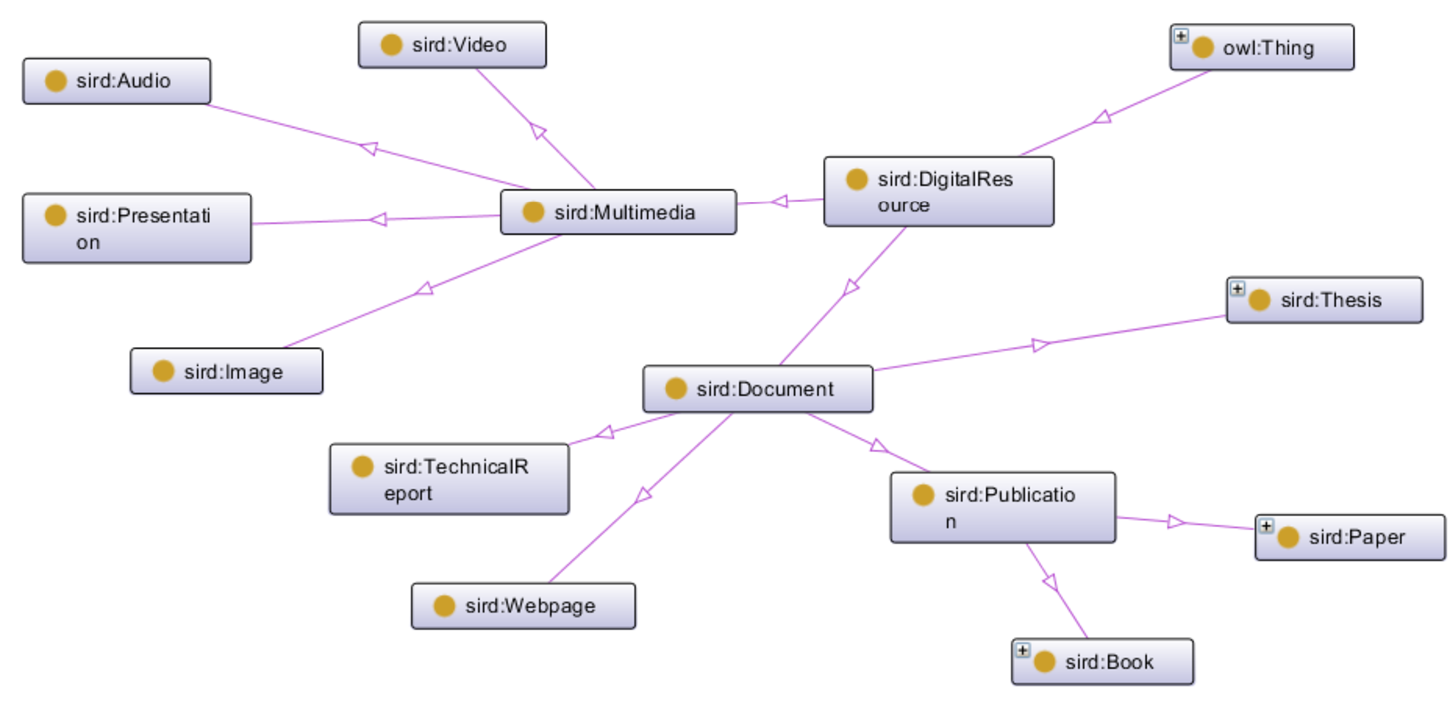
\includegraphics[height=1.8in,width=3.5in]{Clases}
\caption{Class Hierarchy of digital resources in the corporate memory (N\&T) views with prot\'{e}g\'{e}.}
\label{fig:jcl}
\end{figure}

\begin{figure}[!htb]
\centering
%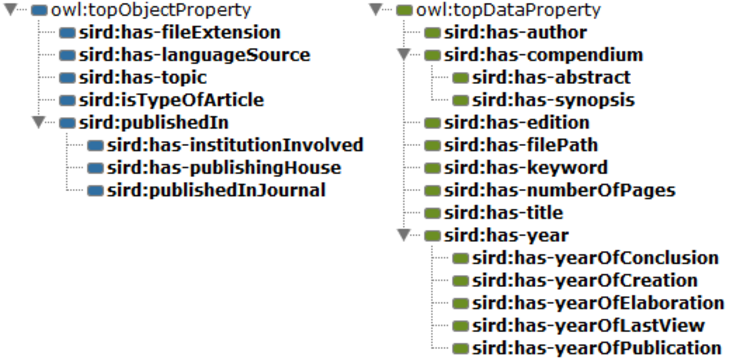
\includegraphics[height=1.7in,width=0.5\textwidth]{Propiedades}
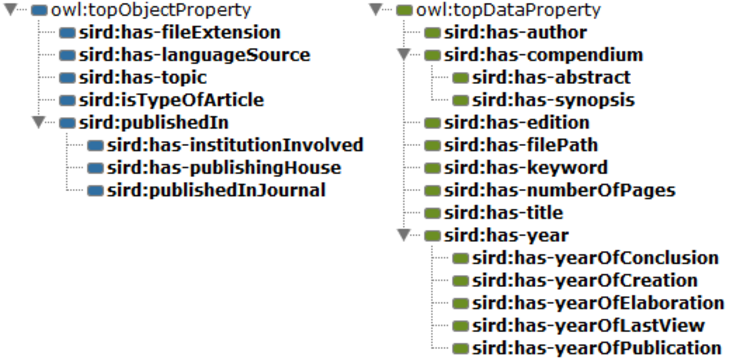
\includegraphics[height=1.4in,width=3in]{Propiedades}
%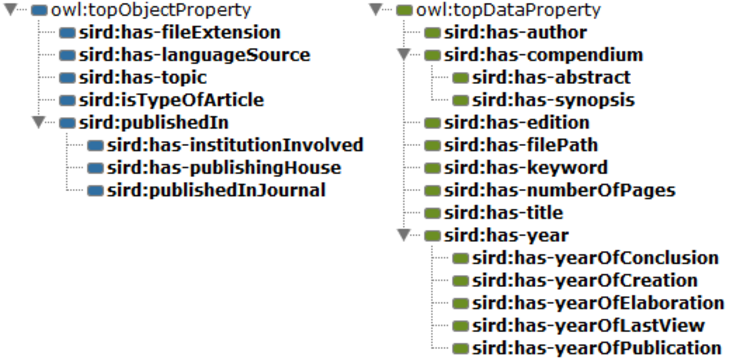
\includegraphics[width=3in]{Propiedades}
\caption{Properties Hierarchy of digital resources in the corporate memory (N\&T) views with prot\'{e}g\'{e}.}
\label{fig:jpr}
\end{figure}

\textbf{Domain and Range}, to set what classes or class-literal, must relate a property (Figure \ref{fig:dyr}.)
\begin{figure}[!htb]
\centering
%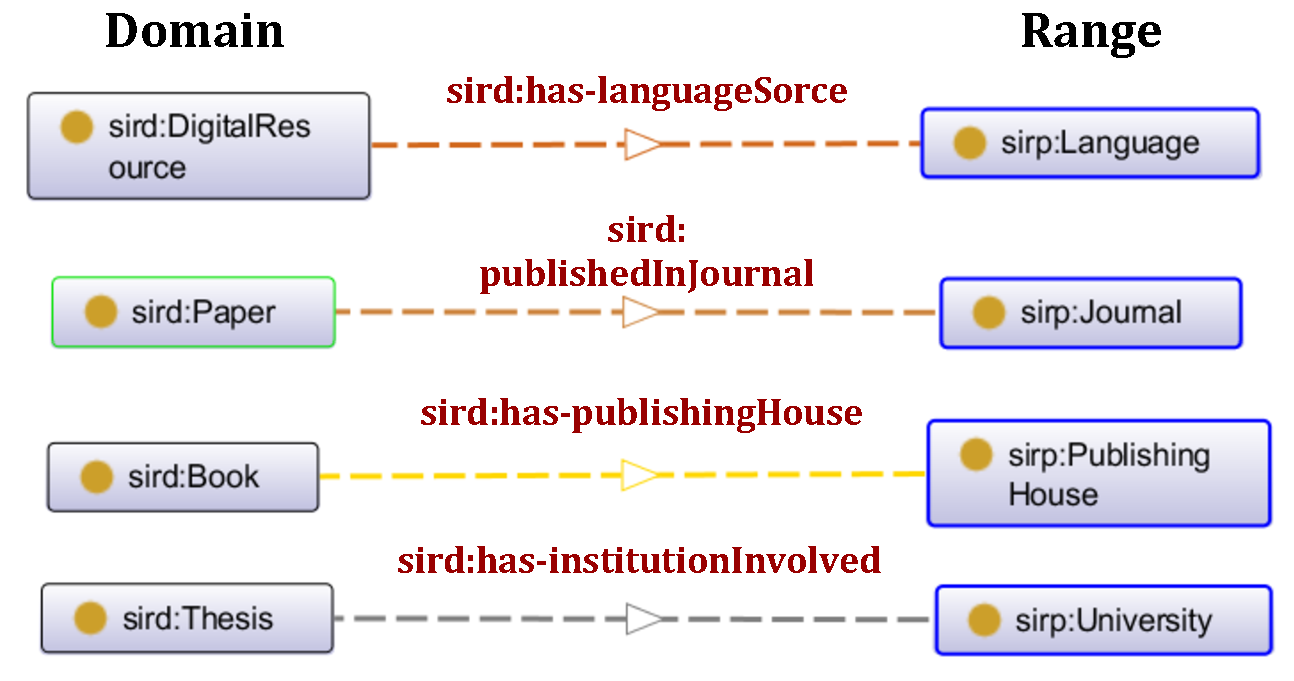
\includegraphics[height=1.8in,width=0.48\textwidth]{DomainyRange}
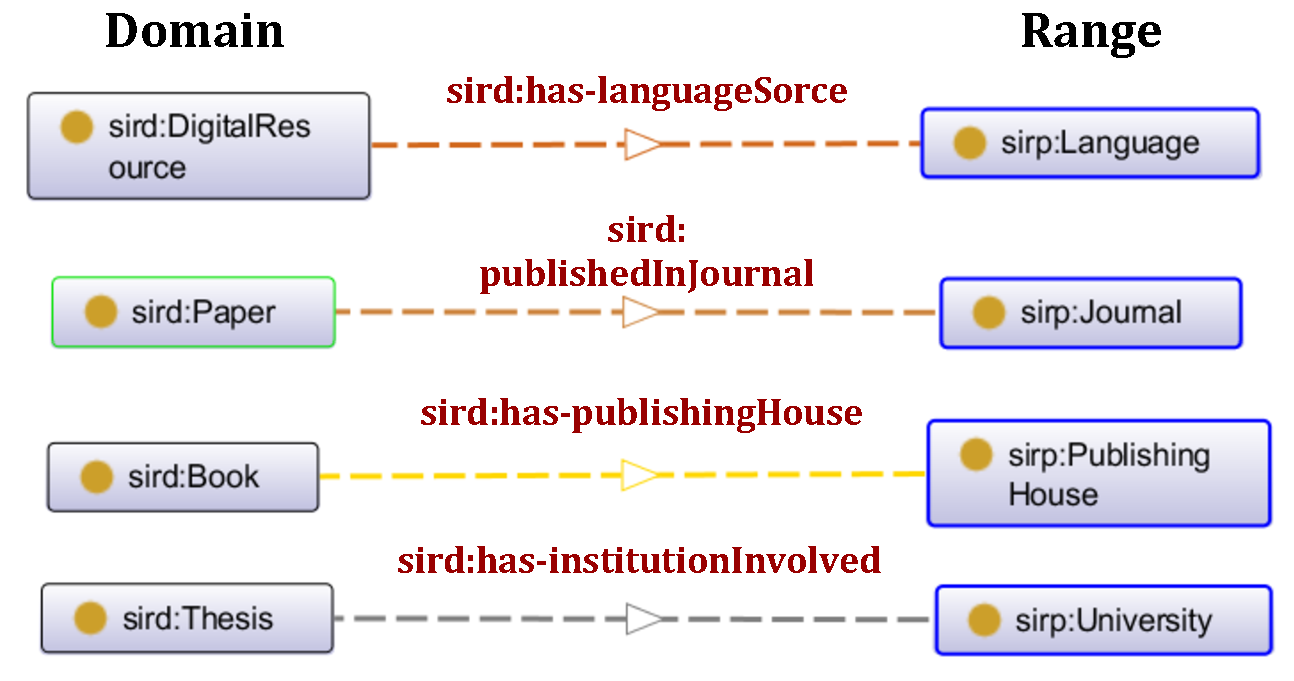
\includegraphics[width=3.5in]{DomainyRange}
\caption{Domain and range of properties of digital resources in the corporate memory (N\&T) views with prot\'{e}g\'{e}.}
\label{fig:dyr}
\end{figure}

There are other axioms, such as: equivalent classes, disjoint classes, property symmetric, transitive property, just to mention. The features and examples of these axioms can find literature \cite{protegeManual}, \cite{Markus2012DLprimer}.

In the same way that the descriptions, the axioms are represented as triples and semantic technologies, standard languages for writing axioms are: RDF Schema (RDF(S) \footnote{W3C,``RDF Vocabulary Description Language 1.0: RDF Schema,'' Available:\url{http://www.w3.org/TR/2004/REC-rdf-
schema-20040210/}}) and Web Ontology Language (OWL\footnote{W3C,``OWL 2 Web Ontology Language Structural Specification and Functional Style Syntax,'' Available: \url{http://www.w3.org/TR/owl2-syntax/}}). There are different tools for writing axioms  in the form of triple with appropriate vocabulary, such as \cite{SurvOnto}, \cite {Buraga2006}: prot�g�, powl, SWOOP, TopBrain, and even to generate triple Jena axioms. In this paper, was elected prot�g� tool because it is a platform that provides a user friendly interface \cite{protege}, allowing it the creation, manipulation and visualization of axioms. In addition, this tool can save axioms in different formats (XML/RDF, Manchester, Turtle, OWL/XML).

The set of axioms that enrich the model is called terminological component (TBox) and semantic technologies, knowledge model consisting of TBox and ABox, is called ontology \cite{Ontoinra2002}. In this proposal, the use cases are independent, therefore, it was decided that each of these has its own ontology. On the other hand, a common goal in both use cases is to link resources with the themes of corporate memory domain. For this, we propose a third ontology which has vocabulary of domain. In our case study, the ontology is the vocabulary of Networks and Telecommunications (N\&T) that developed from another ontology ODARyT \cite{Rios-alvarado_asemantic}. Our ontology vocabulary (ODARyT4sir) consists of 303 items organized into four main branches: Distributed Systems, Networking and Telecommunication, Digital Communication Systems and Semantic Web, and for each concept has its definition. Figure \ref{fig:oda}, shows the four main branches of ODARyT4sir.

\begin{figure}[!htb]
\centering
%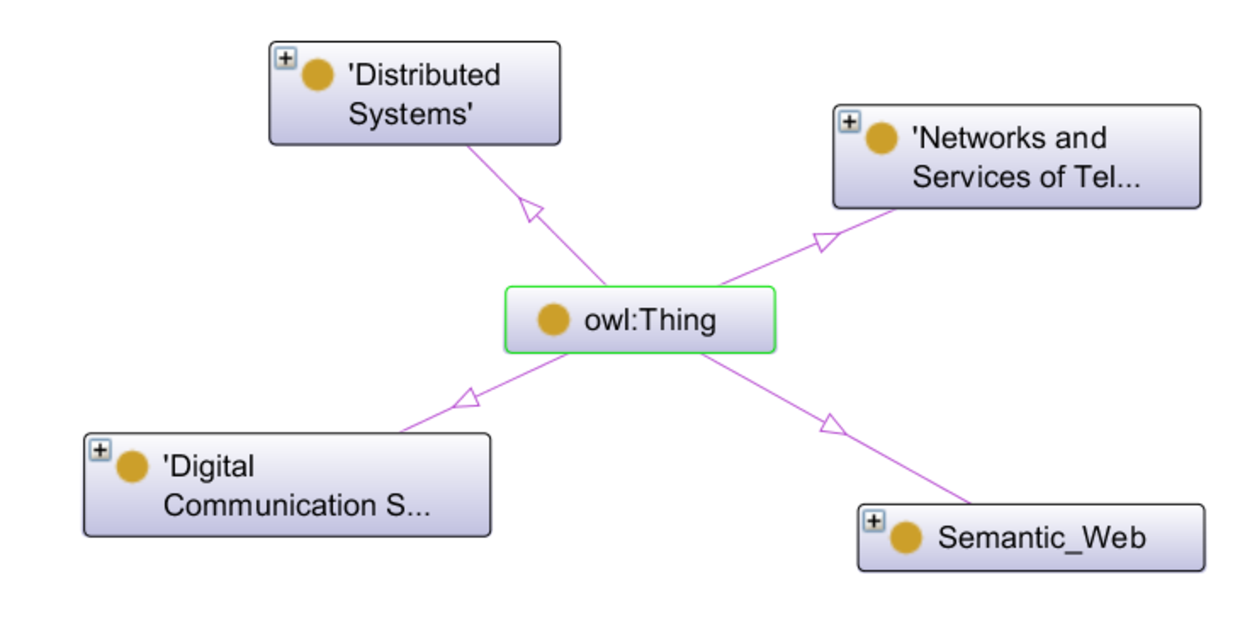
\includegraphics[width=3in]{Odaryt4sir}
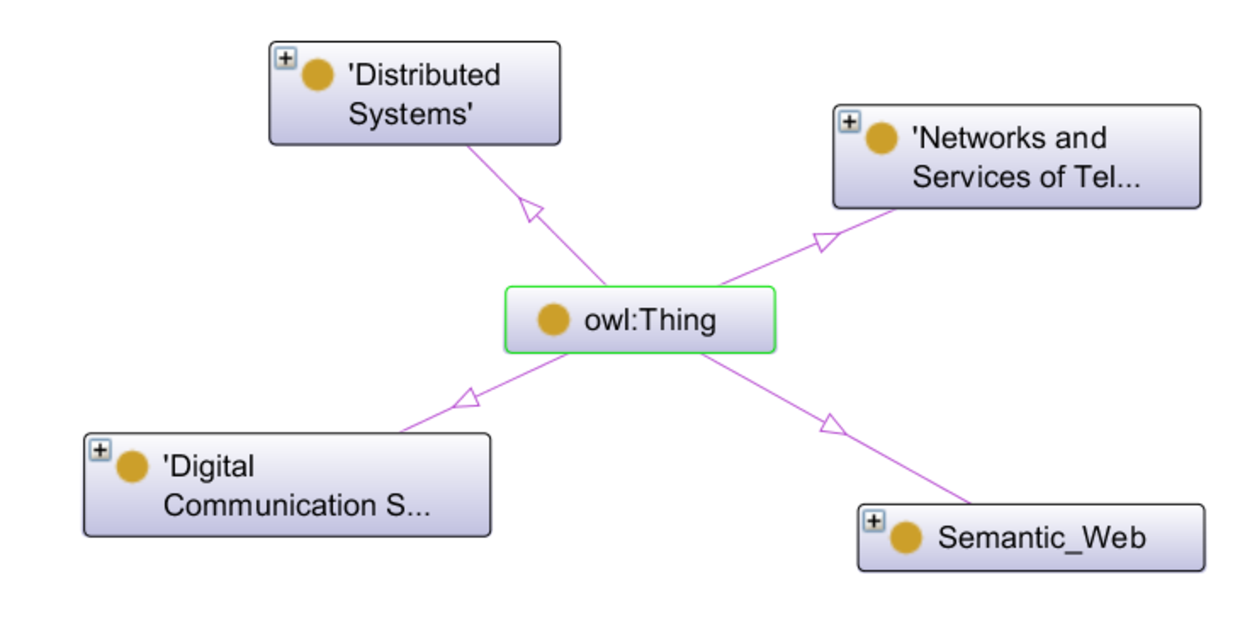
\includegraphics[height=1.2in,width=3in]{Odaryt4sir}
\caption{Ontology with the vocabulary of Networks and Telecommunications (ODARyT4sir) (N\&T) views with prot\'{e}g\'{e}}
\label{fig:oda}
\end{figure}

An ontology has triples on explicit knowledge (resource descriptions) and implicit knowledge (axioms), but the model does not have explicit triples of implicit knowledge. To materialization of this implicit knowledge, uses a reasoner (inference engine) which is a program for inferring facts or associations from existing knowledge (axioms and properties) \cite{InfEng}. For example, we have an ABox with the following description: recourse "Towards a semantic search" is a paper, and TBox with the following axiom: Paper class is a subclass of the Document class, using a reasoner with this ABox and TBox , materializes (inferred) the following description: recourse \textit{Towards a semantic search} is a document. There are different reasoners, such as \cite{InfEng}, \cite{Mishra2011}: Pellet, fact++, racerPro, to name a few. In this paper, we used the reasoner which has by default Jena, because it can be invoked from Java+Jena, supports our ontology axioms (RDF(S) and OWL) and does not require a previous compilation or configuration for use. Furthermore, a reasoner is a tool to validate the model of knowledge, because to find contradictions or ambiguities. In our case study, knowledge models are consistent.

Our ontology of \textit{digital resources} models knowledge of 1330 digital resources. In this model, there are 691 resources which have explicitly assignment triple (rdf: type) to one of the nine basic classes: Durable, Technical Report, Website, Thesis, Book, Audio, Video, Image and Presentation. Meanwhile, the other 639 resources through inference, materializes this triple. Figure \ref{fig:vrc} shows the ontology as venn diagram where the circles are the kinds of Digital Resources and the points are the resources. Meanwhile, Figure \ref{fig:crc} shows cardinality of Venn diagram.

\begin{figure}[!htb]
\centering
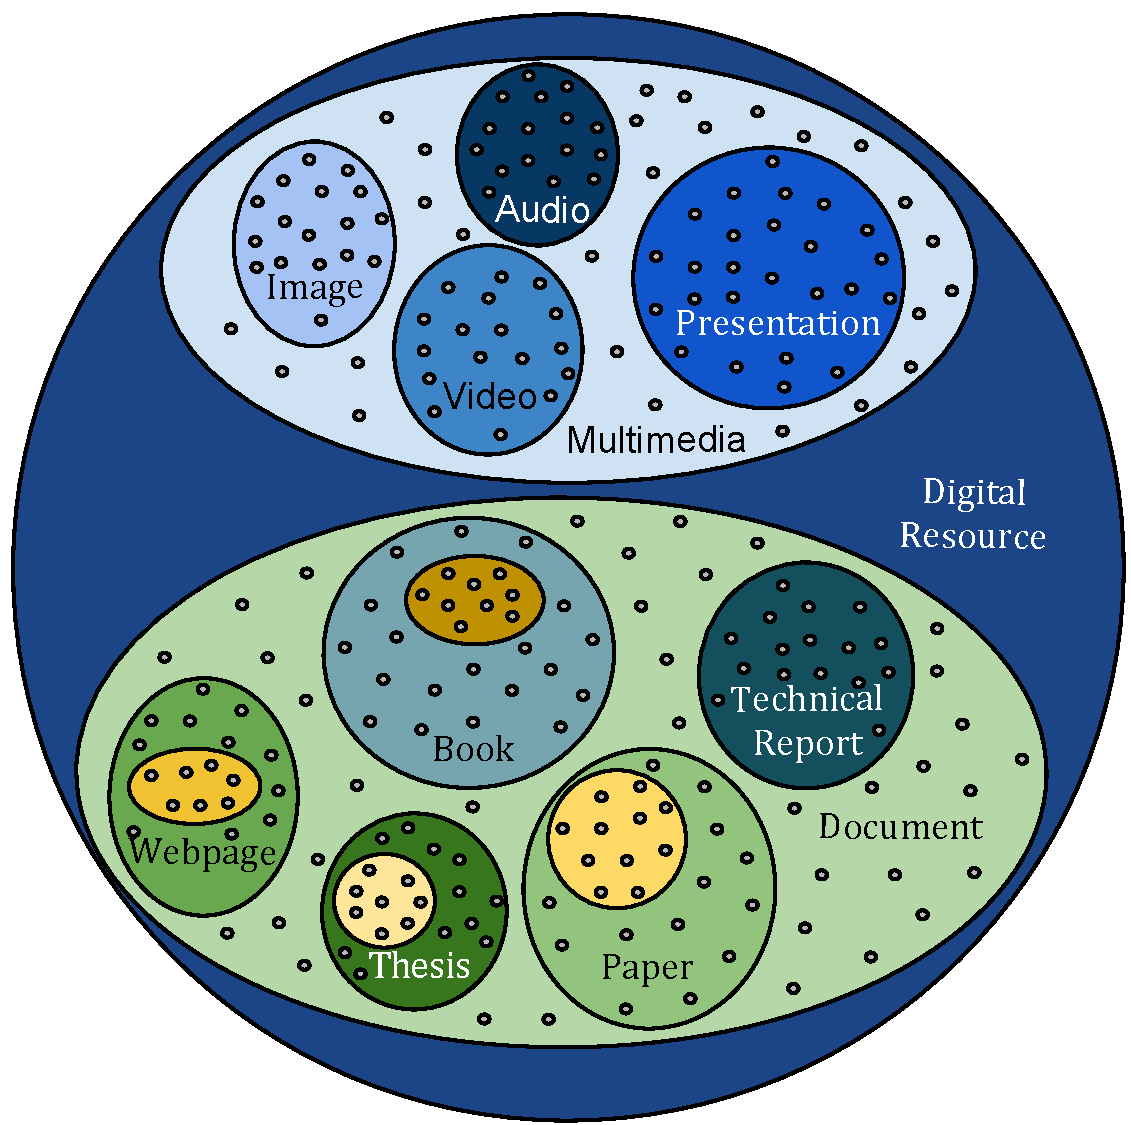
\includegraphics[width=2.7in]{RecDigi}
\caption{Venn diagram of ontology of digital resources by class view.}
\label{fig:vrc}
\end{figure}

\begin{figure}[!htb]
\centering
%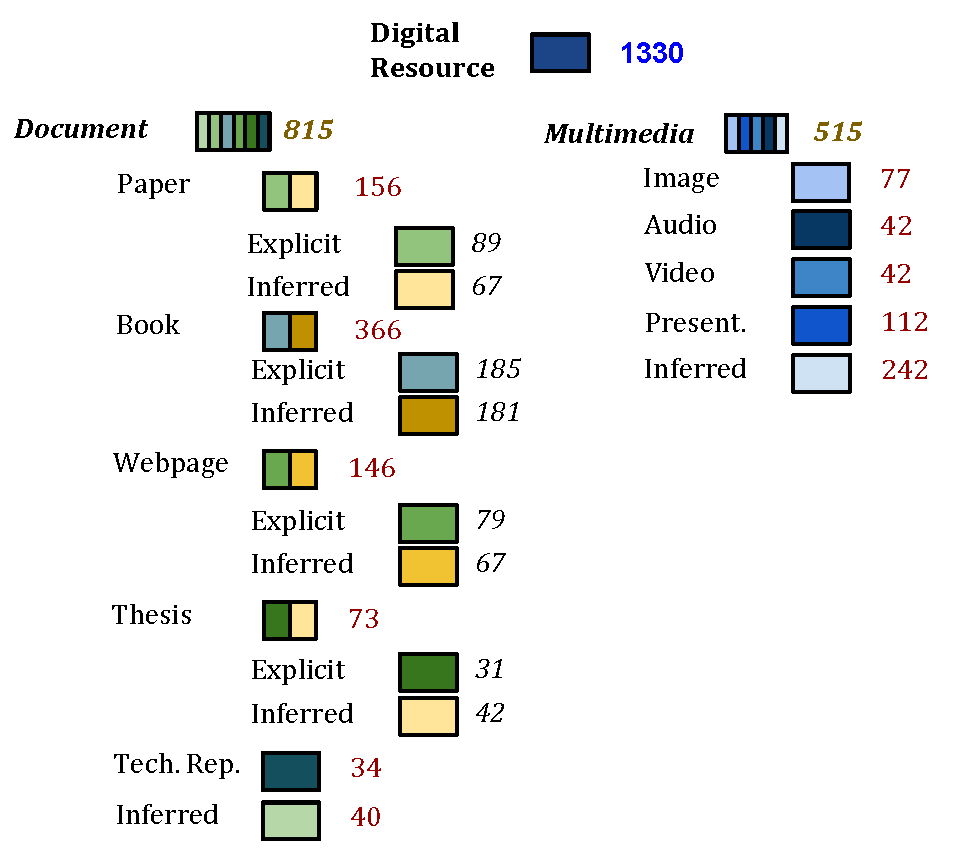
\includegraphics[width=2.5in]{cardinal}
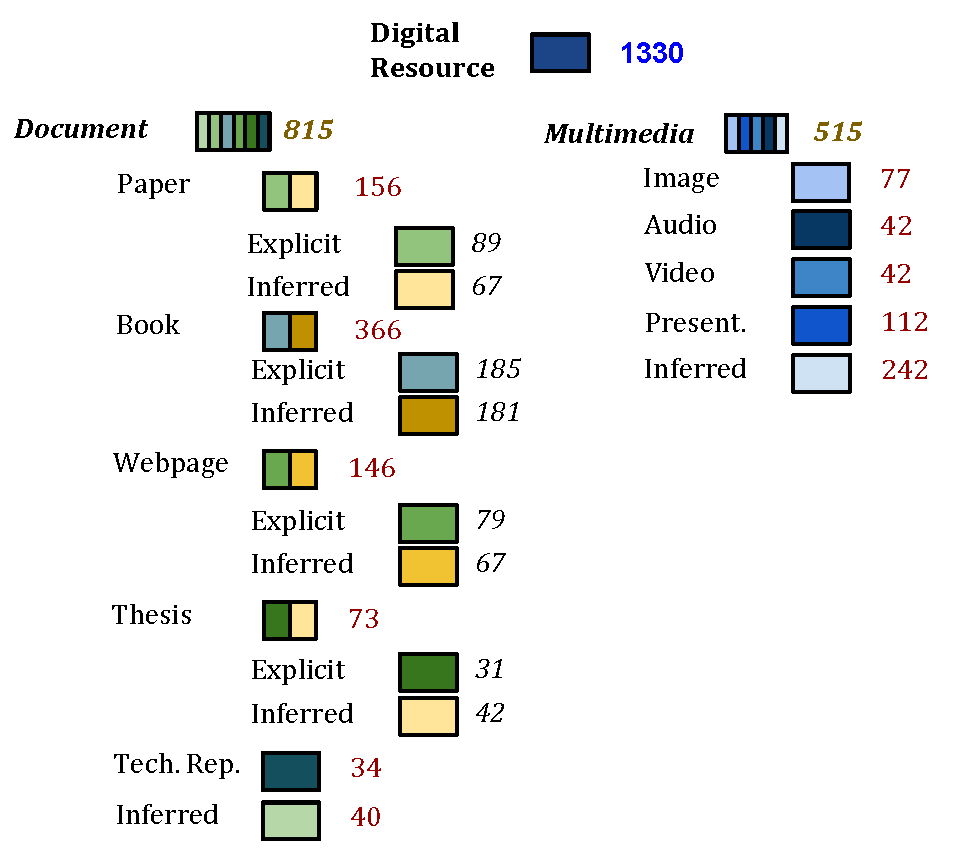
\includegraphics[height=2in,width=2.5in]{cardinal}
\caption{Cardinality of digital resources.}
\label{fig:crc}
\end{figure}

\subsection{Query Information}
\label{sec:cons}
Ontologies are sources of knowledge in form of triples and to integrate information from them, three things are needed:\textit{ 1) a question in natural language, 2) a query from triple and 3) a query engine.}

On the first point, through analysis of use cases are identified and written in natural language the main questions that users can do the model. In our case study, we obtained 10 questions for finding digital resources, but to exemplify the information query, shows one of these: (1) What documents are used to teach a course in P2P Systems?

On the second point, you should use a query language to search and query the triples. In semantic technologies, the language SPARQL\footnote{W3C,``SPARQL 1.1 Overview,'' Available: \url{http://www.w3.org/TR/sparql11-overview/}} \cite{Perez2009} is specification to query, retrieve and modify information of RDF triples. This language is based on the use of search patterns to compare triples model and variables for information retrieval. A search pattern is similar to a triple, but unlike the latter, subject, property or object can be a variable. In a SPARQL query, there are two clauses: SELECT and WHERE. The SELECT clause sets out \textit{outcome variables} and WHERE clause sets out \textit{comparison patterns}. In our example, the question (1) is written as SPARQL query as follows:
\begin{alltt}
\small
SELECT DISTINCT ?title ?path
WHERE
\{?x rdf:type sird:Document;
   sird:has-topic redes:Peer_to_Peer_System;
   sird:has-title ?title;
   sird:has-filePath ?path.\}
\end{alltt}

For third point a SPARQL query engine is a program that can respond to user queries. The basic function of this engine is a SPARQL query interprets, compares triples patterns and model, retrieves information associated with variables that are in SELECT clause and returns information to user. A query engine can be found in triplestore. In particular, Jena has a query engine (ARQ) that supports SPARQL language. This engine ARQ to retrieve results of a query and display on the screen in form of a table or to process these results with JAVA.

\subsection{Prototype (interface User)}
\label{sec:proto}
The semantic integration of resources (SIR) using a triplestore, not a task that any user can do, since it must be familiar with the triplestore and elements of semantic technologies; in particular SPARQL query language and RDF triples. We propose an interface for interaction, transparent and user friendly with triplestore, this interface has the following characteristics:
\begin{itemize}
    \item Browsing through the basic information resource for use case.
    \item Resource specific searches for use case.
    \item Publication of results of search and navigation in a visual format enjoyable.
    \item Mapping the question to a SPARQL query.
    \item Invoking triplestore (load, inference, search) and providing at same the query.
\end{itemize}
In particular, our prototype is a web application interface that works with the triplestore jena, this prototype was implemented in Java and provides a set of servlets that are on a Tomcat server. The prototype provides the following visual interfaces: Browsing through people, Navigation through documents, Navigation through multimedia resources, Advanced people search, Advanced search documents, Multimedia resources advanced search, Advanced search any resource. Figure \ref{fig:moq} shows the interface \textbf{\textit{Navigation through people}}.
\begin{figure}[!htb]
\centering
%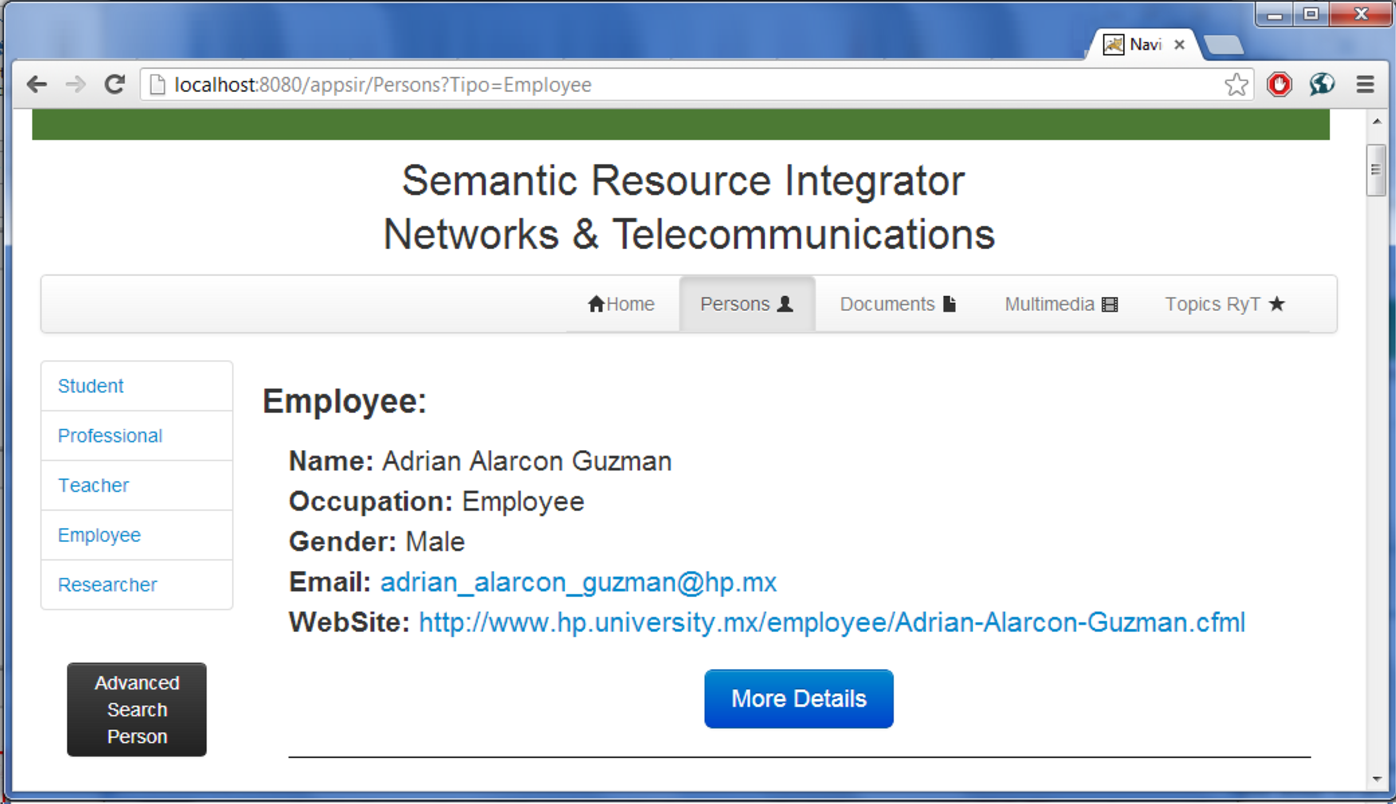
\includegraphics[width=3.5in]{Interfaz}
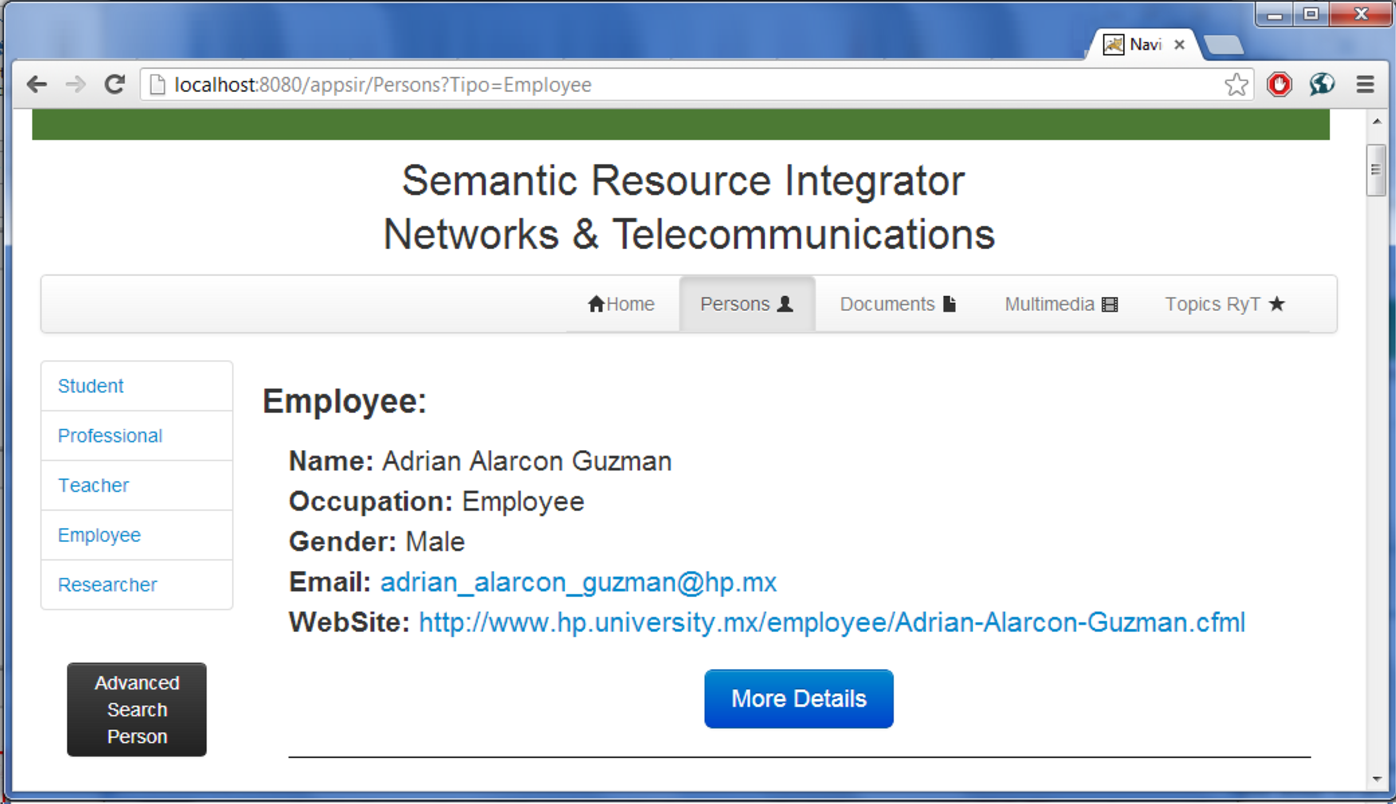
\includegraphics[height=2.2in,width=3.5in]{Interfaz}
\caption{Visual interface navigation through people.}
\label{fig:moq}
\end{figure}

\section{Experimentation}
\label{sec:exp}
In the semantic integration of resources, we have two evaluation criteria for triplestore Jena: \textit{1) performance and 2) the results for a model with inference (reasoner ontology) without inference (explicit descriptions)}. For performance evaluation, we wanted to see if Jena performs adequately with the amount of data that we expect to handle, while for the evaluation of results, we want to see if the results returned by Jena are those who answer our questions.

The performance evaluation involves taking the mean time from model charge, until recovery of results of a query. While the evaluation of results, was to compare information retrieved from a SPARQL query with the resources that are known answer the question (previous analysis). For these two assessments, there was a program in java+jena which repeated \textit{n} times the processing time for a model and a given query, and in each iteration returns the values of the query. The three input parameters of this program are: the number of repetitions, type of model \textit{with explicit data or a reasoner and an ontology} and SPARQL query. Meanwhile, the three output parameters are: average processing time of the consultation, the number of resources that responds the search engine and query responses.

In this paper, we established following parameters for the program: the number of iterations \textit{n} was placed at 20, the models are: 1) the Abox digital resources of N\&T and 2) the ontology digital resources and vocabulary of N\&T, and 3) questions are shown in Table \ref{tab:qln}. This table also shows the number of digital resources that respond to the questions.

\begin{table}[!htb]
\renewcommand{\arraystretch}{1.3}
\caption{Questions in natural language and amount of resources that respond to them}
\label{tab:qln}
\centering
\begin{tabular}{>{\centering\arraybackslash}m{0.4in} >{\arraybackslash}m{2.1in} >{\centering\arraybackslash}m{0.5in}}
\hline 
Id. question & Question & No. of resources\\
\hline
\hline 
Q1 & What are the titles, routes, extension, language, of all digital resources
in N\&T? & 1330. \\
\hline
Q2 & What books are on some topics Distributed Systems? & 103\\
\hline 
Q3 & What resources were published in the UAM? & 18\\
\hline 
Q4 & What documents are to give a course in P2P Systems? & 31\\
\hline 
Q5 & What media resources are greater than 2009? & 119\\
\hline 
Q6 & What documents are about Ontology? & 30\\
\hline 
Q7 & What resources were published in a scientific journal? & 156\\
\hline 
Q8 & What resources are in content the words ``linked data''? & 159\\
\hline 
Q9 & What documents in English and over 2000 are authored by Erik Alarcon
Zamora? & 2\\
\hline 
Q10 & What thesis of Samuel Hernandez Maza? & 4\\
\hline 
\end{tabular}
\end{table}

This program was run on a computer with an Intel Core i7 at 2.3GHz with 8Gb of RAM and 8 processing cores. This test was run using Java 1.7 with integrated development environment Eclipse and Apache Jena 2.7.4 on Windows 7 (64bit). We run the program twice for each question from the list (Table \ref{tab:qln}). The first run, model type is ABox, while in the second run, the model is obtained from the reasoner and ontology. In our case study, the ontology of digital resources has 1330 digital resources and the following amounts of triples: Abox has 20429 and TBox has 107. While vocabulary of N\&T (ODARyT4sir) has 303 concepts and the TBox has 1115 triples. Through inference process and combining both ontologies, we have a total of 38661 triples. The results of measurements of the average time and the number of responses for each query is shown in Table \ref{tab:tnp}.

\begin{table}[!htb]
\renewcommand{\arraystretch}{1.3}
\caption{Average processing time and amount of resources that match a query.}
\label{tab:tnp}
\centering
\begin{tabular}{| >{\centering\arraybackslash}m{0.5in} | >{\centering\arraybackslash}m{0.4in} | >{\centering\arraybackslash}m{0.6in} | >{\centering\arraybackslash}m{0.4in} | >{\centering\arraybackslash}m{0.6in} | }
\hline 
\multirow{2}{*}{Id. question} & \multicolumn{2}{c|}{Model (ABox)} & \multicolumn{2}{c|}{Model (Reasoner+Ontology)}\\
\cline{2-5} 
 & Average Time (ms) & No. of Resources  & Average Time (ms) & No. of Resources\\
\hline 
\hline
Q1 & 12 & 1330/1330 & 138 & 1330/1330\\
\hline
Q2 & 10 & 0/103 & 194 & 103/103\\
\hline
Q3 & 8 & 18/18 & 406 & 18/18\\
\hline
Q4 & 28 & 15/31 & 129 & 31/31\\
\hline
Q5 & 7 & 66/119 & 157 & 119/119\\
\hline
Q6 & 9 & 15/30 & 4016 & 30/30\\
\hline
Q7 & 12 & 156/156 & 3520 & 156/156\\
\hline
Q8 & 16 & 159/159 & 3472 & 159/159\\
\hline
Q9 & 42 & 0/2 & 3451 & 2/2\\
\hline
Q10 & 13 & 3/4 & 3312 & 4/4\\
\hline
\end{tabular}
\end{table}
Table \ref{tab:tnp} shows amount of resources that answer a SPARQL query and to verify that the information in a query answer the question, we did an analysis of the resources that answer each of the questions. Then manually compared information recovered from each SPARQL query with the responses of respective question. In our tests, all results of SPARQL queries are digital resources that we wanted for our questions.

Jena performance is good (less than 1 second) when explicit knowledge is questioned because the query engine directly interrogates the ABox triples. In contrast, Jena consumes more time when model is result of inference, because a reasoner invests time in inference process and if this materializes the triples, then engine compares more triple and invest more time. We think, though Jena does not have a good performance with the use of reasoning, this can be optimized through the use of parallel programming because Jena works with JAVA and can be used processing threads; activity that is outside the scope of this paper.

With respect to the evaluation of information retrieval in two models. On one hand, if the model is the ABox and query is on descriptions, then all query results are expected responses of a question, but if this query is about explicit and implicit knowledge, then several results of question will not be recovered by the ARQ engine. On the other hand, if the model is obtained by the inference in an ontology and the query is about the explicit or implicit, then the ARQ engine is able to recover the expected information for the question. In this way we conclude that despite investing time for inference, we obtained satisfactory results for a user's question.

\section{Conclusion}
\label{sec:concl}
A corporate memory is a source of knowledge to an organization, if this knowledge is represented properly, then the integration of resources will have better results. Our methodology is a generic solution for integrating resource semantics (SIR) which can be implanted in any corporate memory. This methodology is based on two use cases, but is not limited to these, if required adding or changing use cases proposed, then the methodology can be extended to these. We chose semantic technologies for SIR, because it allows: 1) to model, develop and consult knowledge about resources, 2) represent knowledge in a standard format, 3) use tools for developing semantic applications, 4) use and share multiple vocabularies, 5) use applications to exploit the knowledge, among other advantages. Our methodology for integration (SIR) is based on three basic points:   representation, exploitation and consultation of knowledge. In addition to this integration, we developed a prototype for user-friendly and transparent interaction of users with the SIR.

In the performance test of Jena for consultation process, the average time is less than one second when it queries the ABox. But, the time increases (1-3 seconds) when querying a model that was obtained by inference in an ontology. Although the performance of Jena is acceptable for inference model, we believe that using parallel computing operations, these times can be reduced. In the evaluation of information retrieval, using a model that materializes triples, then the results given by Jena are answering the questions we ask. In this way we believe that despite investing time in inference, the results are obtained that satisfies a user's question.

% conference papers do not normally have an appendix


% use section* for acknowledgement
%\section*{Acknowledgment}


%The authors would like to thank\cite{TSW2001}...





% trigger a \newpage just before the given reference
% number - used to balance the columns on the last page
% adjust value as needed - may need to be readjusted if
% the document is modified later
%\IEEEtriggeratref{8}
% The "triggered" command can be changed if desired:
%\IEEEtriggercmd{\enlargethispage{-5in}}

% references section

% can use a bibliography generated by BibTeX as a .bbl file
% BibTeX documentation can be easily obtained at:
% http://www.ctan.org/tex-archive/biblio/bibtex/contrib/doc/
% The IEEEtran BibTeX style support page is at:
% http://www.michaelshell.org/tex/ieeetran/bibtex/
%\bibliographystyle{IEEEtran}
% argument is your BibTeX string definitions and bibliography database(s)
%\bibliography{IEEEabrv,../bib/paper}
%
% <OR> manually copy in the resultant .bbl file
% set second argument of \begin to the number of references
% (used to reserve space for the reference number labels box)

\bibliographystyle{IEEEtran}
\bibliography{IEEEabrv,IEEEref}

%\begin{thebibliography}{1}
%\bibitem{IEEEhowto:kopka}
%H.~Kopka and P.~W. Daly, \emph{A Guide to \LaTeX}, 3rd~ed.\hskip 1em plus
%  0.5em minus 0.4em\relax Harlow, England: Addison-Wesley, 1999.
%\end{thebibliography}




% that's all folks
\end{document}
